\section{Testing and Documentation}
\label{sec:testing_and_documentation}

\subsection{Source-code Testing}

The OpenPRA web application employs an automated and comprehensive testing strategy to ensure the correctness and reliability of its codebase. Static type checking is enforced throughout the front-end, backend, and distributed system components, all of which are implemented in TypeScript, as well as in the scram-node engine, which is written in C++. The use of statically typed languages enables the detection of type-related errors at compile time, thereby reducing the likelihood of runtime failures. In addition to compile-time checks, runtime type validation is performed using a dedicated library, which provides an additional layer of security by preventing invalid or malicious data from propagating through the system.

A continuous integration and deployment (CI/CD) pipeline is established to automate the quality assurance process. Each time a developer pushes code to the remote repository, an automated job is triggered. This job executes a series of static and dynamic tests, including static analysis, code linting, unit tests, and end-to-end tests. The pipeline ensures that the codebase builds correctly and that all tests pass before any changes are merged or deployed. In parallel, the continuous deployment process automatically deploys the application to the target infrastructure, ensuring that the latest validated version is available for use.

Testing in OpenPRA is designed to verify not only the correctness of individual components but also the integrity of their interactions and the stability of the application under evolving requirements and heavy usage. The testing framework encompasses unit, functional, regression, end-to-end, and stress tests, each serving a distinct purpose in the software quality assurance process.

\subsubsection{Unit Testing}

Unit tests are implemented to validate the behavior of isolated components and functions. In the front-end, these tests target interactive elements such as buttons, menus, navigation bars, and text fields, ensuring that user interactions result in the correct manipulation of the Document Object Model (DOM). On the backend, unit tests focus on controller methods, verifying that input parameters and HTTP responses conform to expected behaviors. Within the distributed system, unit tests confirm that quantification jobs are correctly enqueued and managed. The Jest library is used extensively for unit testing in the TypeScript codebase, while the Boost library is employed for unit tests in the C++ scram-node engine.

\subsubsection{Functional Testing}

Functional tests are designed to assess the correct operation of larger application features and their integration. In the front-end, these tests cover workflows such as user registration, authentication, and the use of web editors for constructing fault trees, event trees, event sequence diagrams, and Bayesian networks. Functional testing also verifies that the front-end correctly issues API requests in response to user actions and that the backend services are properly coupled to controllers and can interact with the database and job broker. In the scram-node engine, functional tests ensure that input parameters are correctly propagated through subroutine calls and that error handling mechanisms are effective when processing invalid input data. Figure \ref{fig:test_coverage} shows the functional-test metrics for the web-backend service, indicating the proportion of code covered by the test suite and highlighting sections that may require additional tests.

\subsubsection{Regression Testing}

Regression tests are employed to detect unintended side effects or defects introduced by code modifications. These tests are particularly important for features that are expected to remain stable across releases. For instance, regardless of changes to the graphical representation of models in the web editor, the generated models must always conform to the OpenPRA MEF standard when transmitted via API requests.

\subsubsection{End-to-End Testing}

End-to-end tests simulate complete user workflows, encompassing the entire application stack from the front-end to the backend and distributed system. These tests begin with user account creation, proceed through model construction and quantification, and include subsequent actions such as authentication and model management. The backend is tested for its ability to process quantification requests, interact with the scram-node engine, and manage database operations. The distributed system is evaluated for its ability to coordinate job queuing, processing, and result delivery. Tools such as Playwright and SuperTest are used to automate these scenarios, launching the actual application components and executing predefined sequences of user actions to verify system wide correctness.

\subsubsection{Stress Testing}

Stress testing is conducted to evaluate the application's performance and stability under extreme load conditions. This involves simulating large numbers of concurrent users and repeated execution of end-to-end workflows to identify bottlenecks and establish baseline performance metrics. Stress tests measure parameters such as requests per second, average response time under load, and the maximum sustainable throughput of the backend, job queues, database, and quantification engine. These tests provide critical insights into the system's scalability and resilience.

\subsection{Automated Documentation Generation}

Documentation in OpenPRA is organized to serve both developers and end users. For developers, the documentation provides detailed descriptions of the core functionalities, interfaces, and methods of each component, facilitating quick onboarding and efficient maintenance. For users, the documentation offers guidance on interacting with the front-end, backend, distributed system, and engine as standalone packages, with a focus on API usage and integration.

\subsubsection{HTML-Formatted Documentation}

TSDoc comments are positioned above methods and inside classes across the front-end, back-end, and distributed system codebase to document input parameters, expected types, and output formats. In the C++ scram-node engine, Doxygen-style comments are used to document classes and methods. Inline comments are employed to clarify the use of third-party libraries and APIs, as well as to annotate test cases. Upon compilation, these comments are automatically converted into HTML documentation using tools such as TypeDoc, Compodoc, and Doxygen. The resulting HTML pages are accessible via dedicated URLs, providing a high-level overview of the codebase without requiring direct source code inspection. Figure \ref{fig:html_doc} displays the HTML-formatted documentation for the distributed system microservice, outlining each component’s definition, purpose, and interactions within the broader platform.

\subsubsection{Interactive API Documentation}

The backend and distributed system APIs are documented and made accessible through the Swagger UI \cite{What}, which adheres to the OpenAPI specification. Swagger automatically extracts endpoint definitions, supported operations, input and output schemas, and authentication requirements from the source code. It also allows for the inclusion of metadata such as titles, descriptions, tags, and licensing information. The interactive nature of Swagger enables users to explore and test API endpoints directly from the browser. Responses are returned in a standardized format, combining HTTP status codes with JSON payloads. Figure~\ref{fig:swagger_doc} shows the interactive API documentation generated by Swagger for the distributed system microservice, detailing its available endpoints, supported request methods, and operational descriptions.

\subsection{Documentation for DevOps}

The OpenPRA project adopts DevOps best practices to streamline the software development lifecycle, emphasizing automation, continuous integration, and continuous deployment. Each standalone package, including the front-end, backend, distributed system, database, and scram-engine, is accompanied by dedicated markdown files containing detailed instructions for dependency installation, compilation, package execution, testing, and code formatting. Docker files are provided to automate environment setup and deployment, with comprehensive documentation on containerization workflows. These resources ensure that developers and users have the necessary tools and guidance to effectively develop, deploy, test, and maintain the OpenPRA platform services.
\begin{landscape}
\begin{figure}
    \centering
    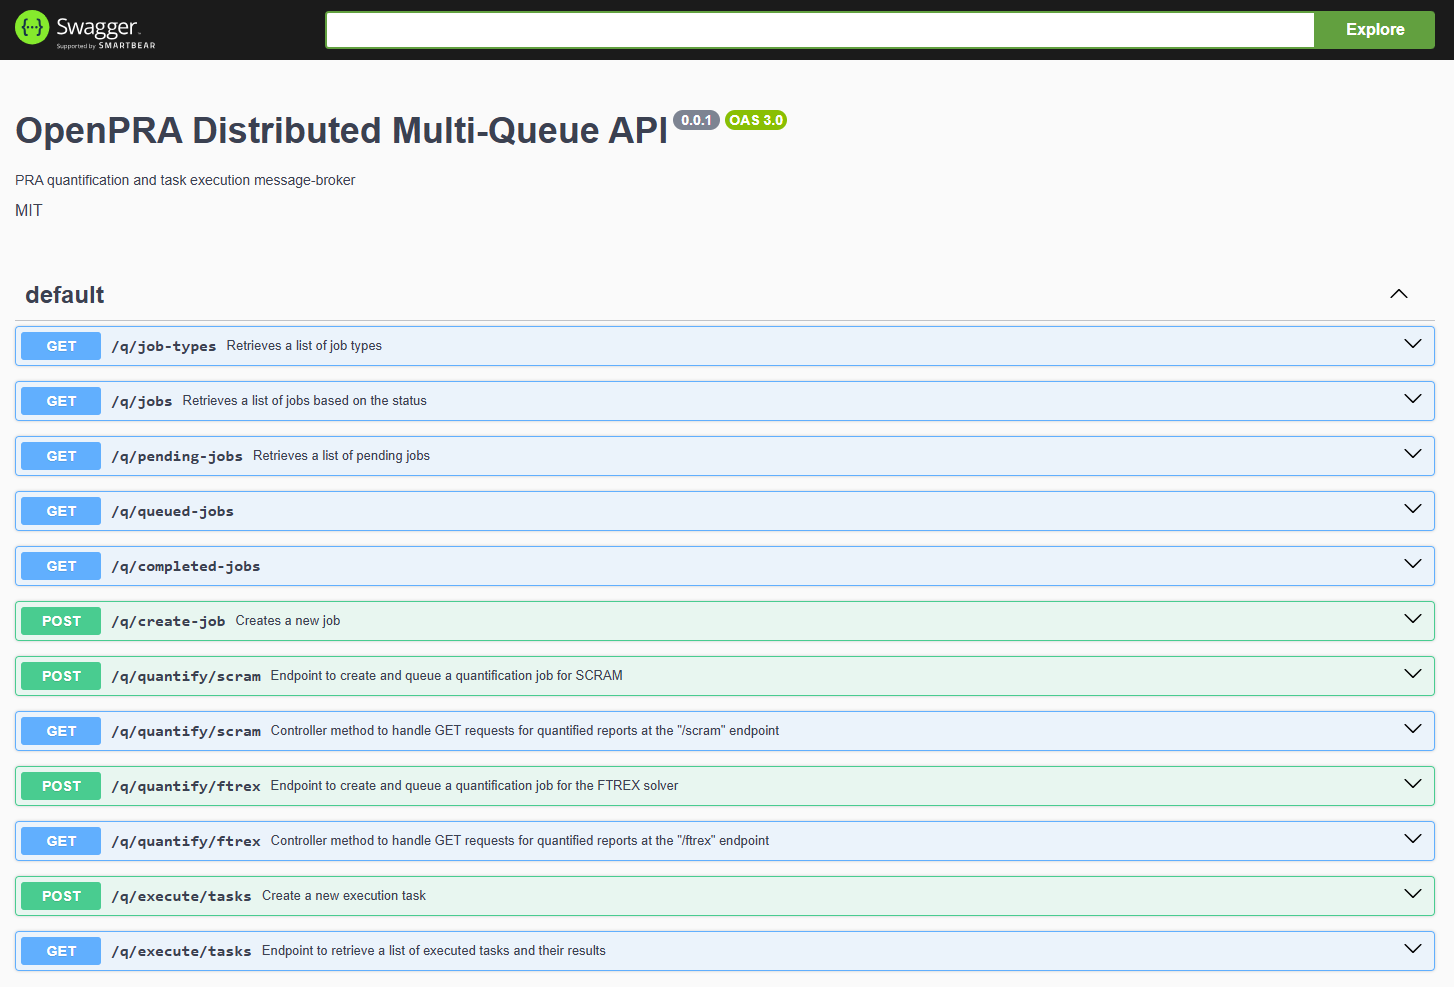
\includegraphics[width=1.3\textwidth]{4_proposed_solution/web_app/figures/swagger_doc.png}
    \caption{Interactive API documentation for the controller of distributed systems microservice.}
    \label{fig:swagger_doc}
\end{figure}
\end{landscape}

\begin{landscape}
\begin{figure}
    \centering
    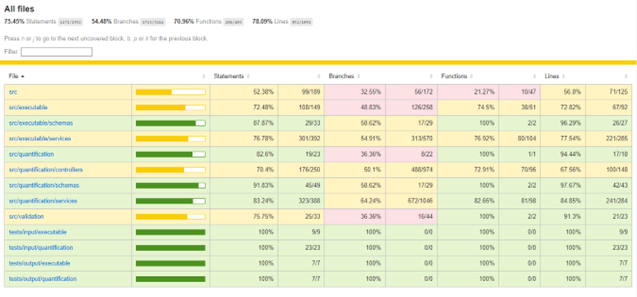
\includegraphics[width=1.3\textwidth]{4_proposed_solution/web_app/figures/test_coverage.png}
    \caption{Test coverage results for the distributed systems microservice.}
    \label{fig:test_coverage}
\end{figure}
\end{landscape}


